\documentclass{standalone}
\usepackage{tikz}
\usetikzlibrary{patterns}
\usetikzlibrary{positioning}
\usetikzlibrary{patterns, positioning}
\usetikzlibrary{shapes.misc}
\usepackage[outline]{contour}
\contourlength{1.5pt} 


\begin{document}
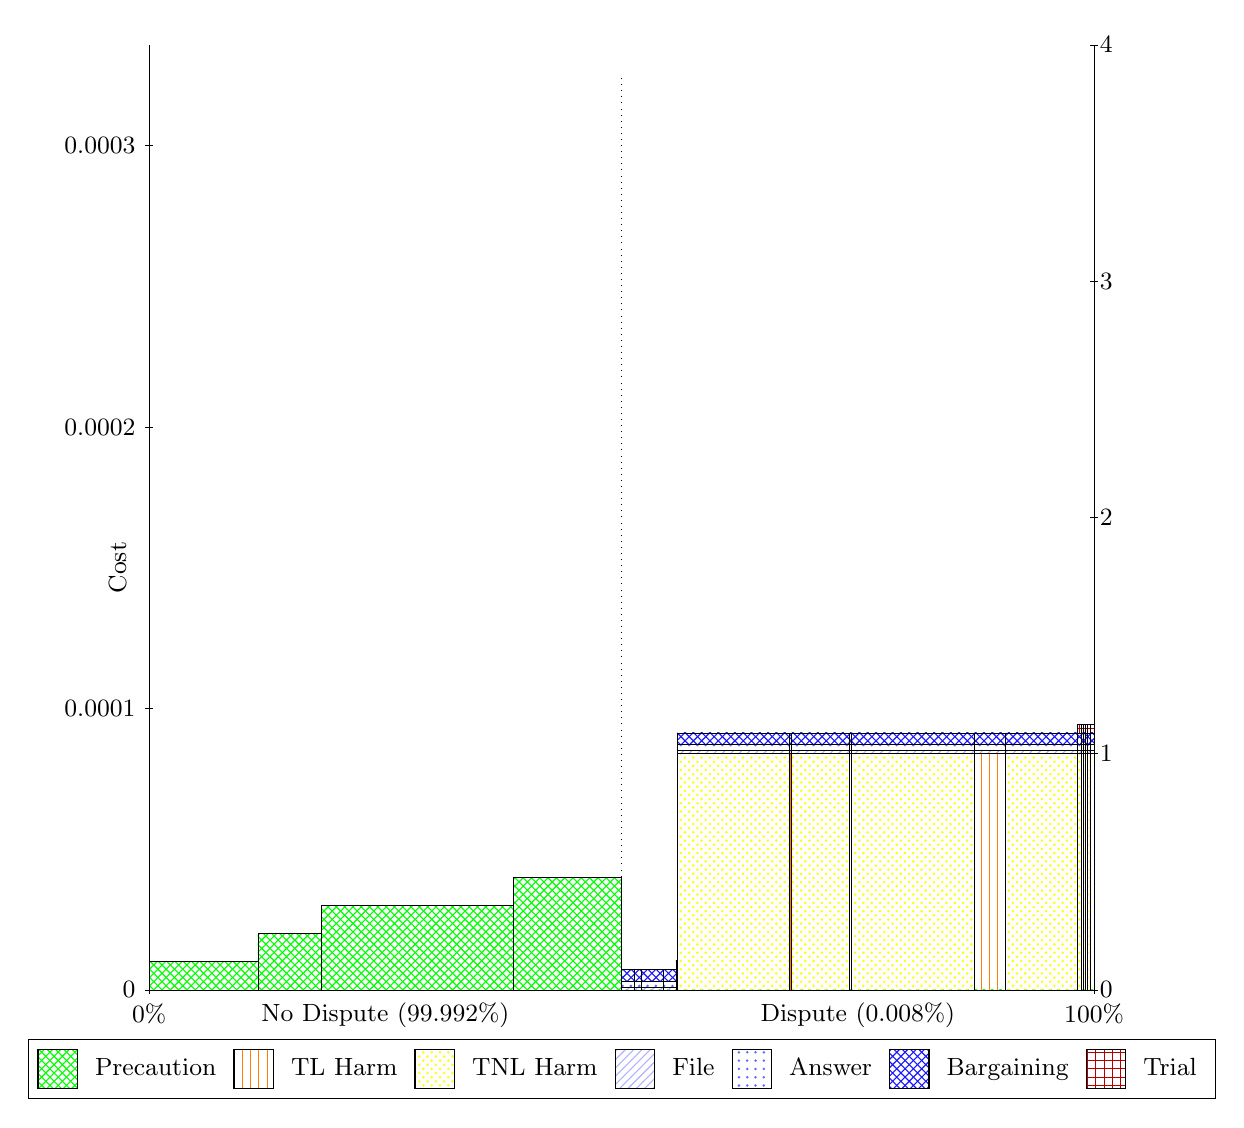
\begin{tikzpicture}
\draw[pattern=crosshatch, pattern color=green,draw=black,very thin] (1.5,2.5) rectangle (2.8801,2.8574);
\draw[pattern=crosshatch, pattern color=green,draw=black,very thin] (2.8801,2.5) rectangle (3.6907,3.2148);
\draw[pattern=crosshatch, pattern color=green,draw=black,very thin] (3.6907,2.5) rectangle (6.1199,3.5722);
\draw[pattern=crosshatch, pattern color=green,draw=black,very thin] (6.1199,2.5) rectangle (7.5,3.9296);
\draw[pattern=crosshatch, pattern color=green,draw=black,very thin] (7.5,2.5) rectangle (7.6559,2.5);
\draw[pattern=north east lines, pattern color=blue!30,draw=black,very thin] (7.5,2.5) rectangle (7.6559,2.5375);
\draw[pattern=dots,  pattern color=blue!60,draw=black,very thin] (7.5,2.5375) rectangle (7.6559,2.6125);
\draw[pattern=crosshatch,      pattern color=blue!90,draw=black,very thin] (7.5,2.6125) rectangle (7.6559,2.7625);
\draw[pattern=crosshatch, pattern color=green,draw=black,very thin] (7.6559,2.5) rectangle (7.747,2.5001);
\draw[pattern=north east lines, pattern color=blue!30,draw=black,very thin] (7.6559,2.5001) rectangle (7.747,2.5376);
\draw[pattern=dots,  pattern color=blue!60,draw=black,very thin] (7.6559,2.5376) rectangle (7.747,2.6126);
\draw[pattern=crosshatch,      pattern color=blue!90,draw=black,very thin] (7.6559,2.6126) rectangle (7.747,2.7626);
\draw[pattern=crosshatch, pattern color=green,draw=black,very thin] (7.747,2.5) rectangle (8.0228,2.5001);
\draw[pattern=north east lines, pattern color=blue!30,draw=black,very thin] (7.747,2.5001) rectangle (8.0228,2.5376);
\draw[pattern=dots,  pattern color=blue!60,draw=black,very thin] (7.747,2.5376) rectangle (8.0228,2.6126);
\draw[pattern=crosshatch,      pattern color=blue!90,draw=black,very thin] (7.747,2.6126) rectangle (8.0228,2.7626);
\draw[pattern=crosshatch, pattern color=green,draw=black,very thin] (8.0228,2.5) rectangle (8.1872,2.5001);
\draw[pattern=north east lines, pattern color=blue!30,draw=black,very thin] (8.0228,2.5001) rectangle (8.1872,2.5376);
\draw[pattern=dots,  pattern color=blue!60,draw=black,very thin] (8.0228,2.5376) rectangle (8.1872,2.6126);
\draw[pattern=crosshatch,      pattern color=blue!90,draw=black,very thin] (8.0228,2.6126) rectangle (8.1872,2.7626);
\draw[pattern=crosshatch, pattern color=green,draw=black,very thin] (8.1872,2.5) rectangle (8.1957,2.5);
\draw[pattern=north east lines, pattern color=blue!30,draw=black,very thin] (8.1872,2.5) rectangle (8.1957,2.5375);
\draw[pattern=dots,  pattern color=blue!60,draw=black,very thin] (8.1872,2.5375) rectangle (8.1957,2.6125);
\draw[pattern=crosshatch,      pattern color=blue!90,draw=black,very thin] (8.1872,2.6125) rectangle (8.1957,2.7625);
\draw[pattern=grid,            pattern color=red!70!black,draw=black,very thin] (8.1872,2.7625) rectangle (8.1957,2.875);
\draw[pattern=crosshatch, pattern color=green,draw=black,very thin] (8.1957,2.5) rectangle (8.2092,2.5001);
\draw[pattern=north east lines, pattern color=blue!30,draw=black,very thin] (8.1957,2.5001) rectangle (8.2092,2.5376);
\draw[pattern=dots,  pattern color=blue!60,draw=black,very thin] (8.1957,2.5376) rectangle (8.2092,2.6126);
\draw[pattern=crosshatch,      pattern color=blue!90,draw=black,very thin] (8.1957,2.6126) rectangle (8.2092,2.7626);
\draw[pattern=grid,            pattern color=red!70!black,draw=black,very thin] (8.1957,2.7626) rectangle (8.2092,2.8751);
\draw[pattern=crosshatch, pattern color=green,draw=black,very thin] (8.2092,2.5) rectangle (9.6242,2.5);
\draw[pattern=crosshatch dots, pattern color=yellow,draw=black,very thin] (8.2092,2.5) rectangle (9.6242,5.5);
\draw[pattern=north east lines, pattern color=blue!30,draw=black,very thin] (8.2092,5.5) rectangle (9.6242,5.5375);
\draw[pattern=dots,  pattern color=blue!60,draw=black,very thin] (8.2092,5.5375) rectangle (9.6242,5.6125);
\draw[pattern=crosshatch,      pattern color=blue!90,draw=black,very thin] (8.2092,5.6125) rectangle (9.6242,5.7625);
\draw[pattern=crosshatch, pattern color=green,draw=black,very thin] (9.6242,2.5) rectangle (9.6536,2.5);
\draw[pattern=vertical lines, pattern color=orange,draw=black,very thin] (9.6242,2.5) rectangle (9.6536,5.5);
\draw[pattern=north east lines, pattern color=blue!30,draw=black,very thin] (9.6242,5.5) rectangle (9.6536,5.5375);
\draw[pattern=dots,  pattern color=blue!60,draw=black,very thin] (9.6242,5.5375) rectangle (9.6536,5.6125);
\draw[pattern=crosshatch,      pattern color=blue!90,draw=black,very thin] (9.6242,5.6125) rectangle (9.6536,5.7625);
\draw[pattern=crosshatch, pattern color=green,draw=black,very thin] (9.6536,2.5) rectangle (10.392,2.5001);
\draw[pattern=crosshatch dots, pattern color=yellow,draw=black,very thin] (9.6536,2.5001) rectangle (10.392,5.5001);
\draw[pattern=north east lines, pattern color=blue!30,draw=black,very thin] (9.6536,5.5001) rectangle (10.392,5.5376);
\draw[pattern=dots,  pattern color=blue!60,draw=black,very thin] (9.6536,5.5376) rectangle (10.392,5.6126);
\draw[pattern=crosshatch,      pattern color=blue!90,draw=black,very thin] (9.6536,5.6126) rectangle (10.392,5.7626);
\draw[pattern=crosshatch, pattern color=green,draw=black,very thin] (10.392,2.5) rectangle (10.418,2.5001);
\draw[pattern=vertical lines, pattern color=orange,draw=black,very thin] (10.392,2.5001) rectangle (10.418,5.5001);
\draw[pattern=north east lines, pattern color=blue!30,draw=black,very thin] (10.392,5.5001) rectangle (10.418,5.5376);
\draw[pattern=dots,  pattern color=blue!60,draw=black,very thin] (10.392,5.5376) rectangle (10.418,5.6126);
\draw[pattern=crosshatch,      pattern color=blue!90,draw=black,very thin] (10.392,5.6126) rectangle (10.418,5.7626);
\draw[pattern=crosshatch, pattern color=green,draw=black,very thin] (10.418,2.5) rectangle (11.972,2.5001);
\draw[pattern=crosshatch dots, pattern color=yellow,draw=black,very thin] (10.418,2.5001) rectangle (11.972,5.5001);
\draw[pattern=north east lines, pattern color=blue!30,draw=black,very thin] (10.418,5.5001) rectangle (11.972,5.5376);
\draw[pattern=dots,  pattern color=blue!60,draw=black,very thin] (10.418,5.5376) rectangle (11.972,5.6126);
\draw[pattern=crosshatch,      pattern color=blue!90,draw=black,very thin] (10.418,5.6126) rectangle (11.972,5.7626);
\draw[pattern=crosshatch, pattern color=green,draw=black,very thin] (11.972,2.5) rectangle (12.375,2.5001);
\draw[pattern=vertical lines, pattern color=orange,draw=black,very thin] (11.972,2.5001) rectangle (12.375,5.5001);
\draw[pattern=north east lines, pattern color=blue!30,draw=black,very thin] (11.972,5.5001) rectangle (12.375,5.5376);
\draw[pattern=dots,  pattern color=blue!60,draw=black,very thin] (11.972,5.5376) rectangle (12.375,5.6126);
\draw[pattern=crosshatch,      pattern color=blue!90,draw=black,very thin] (11.972,5.6126) rectangle (12.375,5.7626);
\draw[pattern=crosshatch, pattern color=green,draw=black,very thin] (12.375,2.5) rectangle (13.29,2.5001);
\draw[pattern=crosshatch dots, pattern color=yellow,draw=black,very thin] (12.375,2.5001) rectangle (13.29,5.5001);
\draw[pattern=north east lines, pattern color=blue!30,draw=black,very thin] (12.375,5.5001) rectangle (13.29,5.5376);
\draw[pattern=dots,  pattern color=blue!60,draw=black,very thin] (12.375,5.5376) rectangle (13.29,5.6126);
\draw[pattern=crosshatch,      pattern color=blue!90,draw=black,very thin] (12.375,5.6126) rectangle (13.29,5.7626);
\draw[pattern=crosshatch, pattern color=green,draw=black,very thin] (13.29,2.5) rectangle (13.341,2.5);
\draw[pattern=crosshatch dots, pattern color=yellow,draw=black,very thin] (13.29,2.5) rectangle (13.341,5.5);
\draw[pattern=north east lines, pattern color=blue!30,draw=black,very thin] (13.29,5.5) rectangle (13.341,5.5375);
\draw[pattern=dots,  pattern color=blue!60,draw=black,very thin] (13.29,5.5375) rectangle (13.341,5.6125);
\draw[pattern=crosshatch,      pattern color=blue!90,draw=black,very thin] (13.29,5.6125) rectangle (13.341,5.7625);
\draw[pattern=grid,            pattern color=red!70!black,draw=black,very thin] (13.29,5.7625) rectangle (13.341,5.875);
\draw[pattern=crosshatch, pattern color=green,draw=black,very thin] (13.341,2.5) rectangle (13.367,2.5);
\draw[pattern=vertical lines, pattern color=orange,draw=black,very thin] (13.341,2.5) rectangle (13.367,5.5);
\draw[pattern=north east lines, pattern color=blue!30,draw=black,very thin] (13.341,5.5) rectangle (13.367,5.5375);
\draw[pattern=dots,  pattern color=blue!60,draw=black,very thin] (13.341,5.5375) rectangle (13.367,5.6125);
\draw[pattern=crosshatch,      pattern color=blue!90,draw=black,very thin] (13.341,5.6125) rectangle (13.367,5.7625);
\draw[pattern=grid,            pattern color=red!70!black,draw=black,very thin] (13.341,5.7625) rectangle (13.367,5.875);
\draw[pattern=crosshatch, pattern color=green,draw=black,very thin] (13.367,2.5) rectangle (13.391,2.5001);
\draw[pattern=crosshatch dots, pattern color=yellow,draw=black,very thin] (13.367,2.5001) rectangle (13.391,5.5001);
\draw[pattern=north east lines, pattern color=blue!30,draw=black,very thin] (13.367,5.5001) rectangle (13.391,5.5376);
\draw[pattern=dots,  pattern color=blue!60,draw=black,very thin] (13.367,5.5376) rectangle (13.391,5.6126);
\draw[pattern=crosshatch,      pattern color=blue!90,draw=black,very thin] (13.367,5.6126) rectangle (13.391,5.7626);
\draw[pattern=grid,            pattern color=red!70!black,draw=black,very thin] (13.367,5.7626) rectangle (13.391,5.8751);
\draw[pattern=crosshatch, pattern color=green,draw=black,very thin] (13.391,2.5) rectangle (13.41,2.5001);
\draw[pattern=vertical lines, pattern color=orange,draw=black,very thin] (13.391,2.5001) rectangle (13.41,5.5001);
\draw[pattern=north east lines, pattern color=blue!30,draw=black,very thin] (13.391,5.5001) rectangle (13.41,5.5376);
\draw[pattern=dots,  pattern color=blue!60,draw=black,very thin] (13.391,5.5376) rectangle (13.41,5.6126);
\draw[pattern=crosshatch,      pattern color=blue!90,draw=black,very thin] (13.391,5.6126) rectangle (13.41,5.7626);
\draw[pattern=grid,            pattern color=red!70!black,draw=black,very thin] (13.391,5.7626) rectangle (13.41,5.8751);
\draw[pattern=crosshatch, pattern color=green,draw=black,very thin] (13.41,2.5) rectangle (13.447,2.5001);
\draw[pattern=crosshatch dots, pattern color=yellow,draw=black,very thin] (13.41,2.5001) rectangle (13.447,5.5001);
\draw[pattern=north east lines, pattern color=blue!30,draw=black,very thin] (13.41,5.5001) rectangle (13.447,5.5376);
\draw[pattern=dots,  pattern color=blue!60,draw=black,very thin] (13.41,5.5376) rectangle (13.447,5.6126);
\draw[pattern=crosshatch,      pattern color=blue!90,draw=black,very thin] (13.41,5.6126) rectangle (13.447,5.7626);
\draw[pattern=grid,            pattern color=red!70!black,draw=black,very thin] (13.41,5.7626) rectangle (13.447,5.8751);
\draw[pattern=crosshatch, pattern color=green,draw=black,very thin] (13.447,2.5) rectangle (13.5,2.5001);
\draw[pattern=vertical lines, pattern color=orange,draw=black,very thin] (13.447,2.5001) rectangle (13.5,5.5001);
\draw[pattern=north east lines, pattern color=blue!30,draw=black,very thin] (13.447,5.5001) rectangle (13.5,5.5376);
\draw[pattern=dots,  pattern color=blue!60,draw=black,very thin] (13.447,5.5376) rectangle (13.5,5.6126);
\draw[pattern=crosshatch,      pattern color=blue!90,draw=black,very thin] (13.447,5.6126) rectangle (13.5,5.7626);
\draw[pattern=grid,            pattern color=red!70!black,draw=black,very thin] (13.447,5.7626) rectangle (13.5,5.8751);
\draw[black,very thin] (1.5,2.5) -- (1.5,14.5);
\node[font=\small,rotate=90,text=black, anchor=center] at (1.1, 7.8608) {Cost};
\draw[black,very thin] (1.45,2.5) -- (1.55,2.5);
\node[font=\small,text=black, anchor=east] at (1.45, 2.5) {0};
\draw[black,very thin] (1.45,6.0739) -- (1.55,6.0739);
\node[font=\small,text=black, anchor=east] at (1.45, 6.0739) {0.0001};
\draw[black,very thin] (1.45,9.6478) -- (1.55,9.6478);
\node[font=\small,text=black, anchor=east] at (1.45, 9.6478) {0.0002};
\draw[black,very thin] (1.45,13.222) -- (1.55,13.222);
\node[font=\small,text=black, anchor=east] at (1.45, 13.222) {0.0003};

\draw[black,dotted,very thin] (7.5,2.86) -- (7.5,14.14);
\draw[black,very thin] (13.5,2.5) -- (13.5,14.5);
\draw[black,very thin] (13.45,2.5) -- (13.55,2.5);
\node[font=\small,text=black, anchor=west] at (13.45, 2.5) {0};
\draw[black,very thin] (13.45,5.5) -- (13.55,5.5);
\node[font=\small,text=black, anchor=west] at (13.45, 5.5) {1};
\draw[black,very thin] (13.45,8.5) -- (13.55,8.5);
\node[font=\small,text=black, anchor=west] at (13.45, 8.5) {2};
\draw[black,very thin] (13.45,11.5) -- (13.55,11.5);
\node[font=\small,text=black, anchor=west] at (13.45, 11.5) {3};
\draw[black,very thin] (13.45,14.5) -- (13.55,14.5);
\node[font=\small,text=black, anchor=west] at (13.45, 14.5) {4};

\draw[black,very thin] (1.5,2.5) -- (13.5,2.5);
\draw[black,very thin] (1.5,2.45) -- (1.5,2.55);
\node[font=\small,text=black, anchor=north] at (1.5, 2.45) {0\%};
\draw[black,very thin] (13.5,2.45) -- (13.5,2.55);
\node[font=\small,text=black, anchor=north] at (13.5, 2.45) {100\%};

\node[font=\small,text=black,anchor=south] at (4.5, 1.9) {No\ Dispute\ (99.992\%)};
\node[font=\small,text=black,anchor=south] at (10.5, 1.9) {Dispute\ (0.008\%)};
\draw (7.5,2.5) node (B) {};
\begin{scope}[align=center]
\matrix[scale=0.5,draw=black,below=0.5cm of B,nodes={draw},column sep=0.1cm]{
\node[rectangle,draw,minimum width=0.5cm,minimum height=0.5cm,pattern=crosshatch, pattern color=green]{}; & \node[draw=none,font=\small,text=black]{Precaution}; &
\node[rectangle,draw,minimum width=0.5cm,minimum height=0.5cm,pattern=vertical lines, pattern color=orange]{}; & \node[draw=none,font=\small,text=black]{TL Harm}; &
\node[rectangle,draw,minimum width=0.5cm,minimum height=0.5cm,pattern=crosshatch dots, pattern color=yellow]{}; & \node[draw=none,font=\small,text=black]{TNL Harm}; &
\node[rectangle,draw,minimum width=0.5cm,minimum height=0.5cm,pattern=north east lines, pattern color=blue!30]{}; & \node[draw=none,font=\small,text=black]{File}; &
\node[rectangle,draw,minimum width=0.5cm,minimum height=0.5cm,pattern=dots,  pattern color=blue!60]{}; & \node[draw=none,font=\small,text=black]{Answer}; &
\node[rectangle,draw,minimum width=0.5cm,minimum height=0.5cm,pattern=crosshatch,      pattern color=blue!90]{}; & \node[draw=none,font=\small,text=black]{Bargaining}; &
\node[rectangle,draw,minimum width=0.5cm,minimum height=0.5cm,pattern=grid,            pattern color=red!70!black]{}; & \node[draw=none,font=\small,text=black]{Trial}; \\\\
};\end{scope}

\end{tikzpicture}
\end{document}